\documentclass[10pt]{beamer}
%\documentclass[handout]{beamer}
%\usepackage{xeCJK}

%\usepackage[orientation=landscape,size=custom,width=16,height=12,scale=0.5,debug]{beamerposter}
\usepackage{ctex}

 % 1. packages

 % ----------- fonts and symbles ---------
\usepackage{amsmath,amssymb,amsfonts,amsthm}
%\usepackage{CJK}
\usepackage{dsfont}
\usepackage{mathrsfs}
\usepackage{eucal} % for \mathcal

%\renewcommand{\rmdefault}{ptm}


%\usepackage{fontspec}
%\newfontfamily\monaco{Monaco}

%\usepackage{mathbbold} %,bbold

 \usepackage{textcomp} % for \textnormal{\textperthousand}
% -----------------





%\usepackage{slashbox}
%\usepackage[margin=2.2cm]{geometry} % |geometry| package clash with |booktabs| package
%\usepackage{cases}
% -------- tables -------
\usepackage{booktabs} % for \toprule, \bottomrule
\usepackage{tabularx}
\usepackage{multirow}
% --------- figures ---------
\usepackage{graphicx}
% ---------- algorithms -------
\usepackage{algorithm}
\usepackage{algorithmic}
%\usepackage{footnote}
    % |footnote| package occurs error:
    % Runaway argument?
    % \def \insertfootnotetext {\@@ }\def \insertfootnotemark {\@makefnmark \ETC.

\usepackage{listings}

\usepackage[linewidth=1pt]{mdframed} % for  mdframe environment




 \usepackage{color}
 \usepackage{xcolor}     %¸ßÁÁʹÓõÄÑÕÉ«

\usepackage{setspace}
%%\usepackage{type1cm}
\usepackage{adjustbox} % for \adjustbox

\usepackage{accsupp}
\newcommand{\emptyaccsupp}[1]{\BeginAccSupp{ActualText={}}#1\EndAccSupp{}}




%%   figures and tables
\graphicspath{{figure/}}


% 2. new commands

% 2.0 common commands
%\newcommand{\bc}{\begin{center}}
%\newcommand{\ec}{\end{center}}
%\newcommand{\ba}{\begin{array}}
%\newcommand{\ea}{\end{array}}
%\newcommand{\be}{\begin{equation}}
%\newcommand{\ee}{\end{equation}}

% 2.1 colors
\definecolor{dgrey}{rgb}{0.30,0.30,0.30}
\definecolor{lred}{rgb}{0.50,0.00,0.50}
\definecolor{lblue}{rgb}{0.8,0.8,1}
\definecolor{dred}{rgb}{0.6,0,0}
\definecolor{dblue}{rgb}{0,0,0.5}
\definecolor{dgrey}{rgb}{0.35,0.35,0.35}
\definecolor{rred}{rgb}{0.9,0,0}
\definecolor{mylblue}{rgb}{0.3,0.2, 0.8}

\definecolor{commentcolor}{RGB}{85,139,78}
\definecolor{stringcolor}{RGB}{206,145,108}
\definecolor{keywordcolor}{RGB}{34,34,250}
\definecolor{backcolor}{RGB}{220,220,220}

\newcommand{\blue}[1]{{\color{blue}#1}}
\newcommand{\dblue}[1]{{\color{dblue}#1} }
\newcommand{\red}[1]{{\color{red}#1}}
\newcommand{\dred}[1]{{\color{dred}#1}}
\newcommand{\cyan}[1]{{\color{cyan}#1}}
\newcommand{\bfblue}[1]{\textbf{\color{dblue}#1} }
\newcommand{\bfred}[1]{\textbf{\color{dred}#1} }
\newcommand{\green}[1]{{\color{green}#1}}
%\newcommand{\alert}[1]{{\color{red}#1}}
\newcommand{\black}[1]{{\color{black}#1}}
\newcommand{\light}[1]{{\color{blue}\textbf{#1}}}
\newcommand{\hot}[1]{{\color{dred}#1}}
 \newcommand{\highlight}[1]{ \textbf{\color{mylblue}#1}}
 \newcommand{\important}[1]{{\color{red}#1}} % for highlighting  some words

 \newcommand{\mystar}{\dred{$^{\clubsuit}$ }}
  \newcommand{\doublestar}{\dred{$^{\clubsuit\clubsuit}$ }}

\newcommand{\mynote}[1]{{\footnotesize \color{mylblue}#1}}

 \newcommand{\hint}[1]{{\small \color{mylblue}#1}}
\newcommand{\smallhint}[1]{{\small \color{dgrey}#1}}
\newcommand{\footnotehint}[1]{{\footnotesize \color{dgrey}#1}}
\newcommand{\tinyhint}[1]{{\tiny \color{dgrey}#1}}
\newcommand{\mytitle}[1]{\medskip{\large \textbf{\color{mylblue}#1}}}
\newcommand{\normaltitle}[1]{\medskip{ \textbf{\color{mylblue}#1}}}

%\newcommand{\head}[1]{\textbf{\large\color{blue}#1}}
%\newcommand{\heading}[1]{\textbf{\large\color{blue}#1}}

\newcommand{\myfbox}[2]{ \bigskip \begin{center} \fbox{\parbox{#1}{ #2  }} \end{center}\bigskip }

\newcommand{\myvar}[1]{}
%\newcommand{\mynote}[1]{#1}

% 2.2 mathematical symbols

\newcommand{\drightarrow}{\stackrel{d.}{\rightarrow}}
\newcommand{\prightarrow}{\stackrel{p.}{\rightarrow}}
\newcommand{\bernoulli}{\textnormal{Ber}}
\newcommand{\cov}{\mathsf{Cov}}
\newcommand{\corr}{\mathbf{Corr}}
\newcommand{\regret}{\textnormal{Regret}}
\newcommand{\conv}{\textnormal{conv}}
\newcommand{\dotdiv}{\stackrel{\centerdot}{-}}
\newcommand{\dom}{\textnormal{dom}}
\newcommand{\convergenceinprob}{\stackrel{P}{\rightarrow}}
\newcommand{\convergenceindist}{\rightsquigarrow}
\newcommand{\probability}{\mathbb{P}}
\newcommand{\expectation}{\mathbb{E}}
\newcommand{\epi}{\textnormal{epi}}
\newcommand{\variance}{\mathbb{V}}
\newcommand{\var}[1]{\mathbb{V}(#1)}
\newcommand{\covariance}{\mathsf{Cov}}
\newcommand{\empiricalrisk}[1]{\hat{R}(#1)}
\newcommand{\expectedrisk}[1]{R(#1)}
\newcommand{\mgf}[1]{\psi_{#1}(\lambda)}
\newcommand{\mgfexpansion}[1]{\expectation[e^{\lambda#1}]}
\newcommand{\mgfmultivariate}[1]{\expectation[e^{\lambda^\transpose#1}]}
\newcommand{\transpose}{{\mathsf{T}}}
\newcommand{\real}{\mathbb{R}}
\newcommand{\gaussian}[2]{\mathcal{N}(#1,#2)}
\newcommand{\subGaussian}[1]{\mathsf{subG}(#1)}
\newcommand{\indicator}[1]{\mathbb{I}[#1]}
\newcommand{\x}[1]{x^{(#1)}}
\newcommand{\y}[1]{y^{(#1)}}
\newcommand{\z}[1]{z^{(#1)}}
\newcommand{\feature}{x}
\newcommand{\response}{y}
\newcommand{\supofempiricalprocess}{\|\mathbb{P}_n-\mathbb{P}\|_{\decisionspace}}
\newcommand{\decisionspace}{\mathscr{F}}
\newcommand{\decisionfunction}{f}
\newcommand{\featurespace}{\mathcal{X}}
\newcommand{\classifierestimate}{\widehat{h}}
\newcommand{\classifiertrue}{h^\star}
\newcommand{\classifier}{h}
\newcommand{\hypothesisclass}{\mathcal{H}}
\newcommand{\dataset}{\mathcal{D}}
\newcommand{\defineas}{\stackrel{\textnormal{def}}{=}}
\newcommand{\rademachercomplexity}[1]{\mathsf{Rad}_n\left(#1\right)}
\newcommand{\loss}{\ell}
\newcommand{\composite}{\circ}
\newcommand{\convexhull}{\mathsf{conv}}
\newcommand{\norm}[2][2]{\|#2\|_{#1}}
\newcommand{\shatteringcoefficient}[2]{\mathcal{S}(#1,#2)}
\newcommand{\vcdimension}[1]{\mathsf{VC}\left(#1\right)}
\newcommand{\rank}{\mathsf{rank}}
\newcommand{\innerproduct}[2]{\left\langle #1, #2\right\rangle}
\newcommand{\modelparameter}{\theta}
\newcommand{\ball}[3][]{\mathcal{B}_{{#1}}\left(#2,#3\right)}
\newcommand{\metric}{d}
\newcommand{\coveringnumber}[4][]{N_{{#1}}\left(#2,#3,#4\right)}
\newcommand{\trace}{\textnormal{tr}}
\newcommand{\std}{\textnormal{std}}
\newcommand{\sgn}{\textnormal{sign}}
%\renewcommand{\span}{\textnormal{span}}

 % do not overwrite the existing command \span
 % as it leads to an error of
 %  "Missing # Inserted in Alignment Preamble" for ``align'' environment

\newcommand{\myspan}{\textnormal{span}}

%%%
\newcommand{\rightarrowd}{\stackrel{d}{\rightarrow}}
\newcommand{\rightarrowp}{\stackrel{p}{\rightarrow}}
\newcommand{\defeq}{ \stackrel{\textnormal{def}}{=}}
\newcommand{\proj}{ \textnormal{Proj}}
\newcommand{\dist}{\textnormal{dist}}

\newcommand{\argmax}{\textnormal{argmax}}
\newcommand{\argmin}{\textnormal{argmin}}
\newcommand{\subg}{\textnormal{subG}}


 \newcommand{\bba}{\mathbb{A}}
\newcommand{\bbb}{\mathbb{B}}
\newcommand{\bbc}{\mathbb{C}}
\newcommand{\bbd}{\mathbb{D}}
\newcommand{\bbe}{\mathbb{E}}
\newcommand{\bbf}{\mathbb{F}}
\newcommand{\bbg}{\mathbb{G}}
\newcommand{\bbh}{\mathbb{H}}
\newcommand{\bbi}{\mathbb{I}}
\newcommand{\bbj}{\mathbb{J}}
\newcommand{\bbk}{\mathbb{K}}
\newcommand{\bbl}{\mathbb{L}}
\newcommand{\bbm}{\mathbb{M}}
\newcommand{\bbn}{\mathbb{N}}
\newcommand{\bbo}{\mathbb{O}}
\newcommand{\bbp}{\mathbb{P}}
\newcommand{\bbq}{\mathbb{Q}}
\newcommand{\bbr}{\mathbb{R}}
\newcommand{\bbs}{\mathbb{S}}
\newcommand{\bbt}{\mathbb{T}}
\newcommand{\bbu}{\mathbb{U}}
\newcommand{\bbv}{\mathbb{V}}
\newcommand{\bbw}{\mathbb{W}}
\newcommand{\bbx}{\mathbb{X}}
\newcommand{\bby}{\mathbb{Y}}
\newcommand{\bbz}{\mathbb{Z}}

\newcommand{\bfa}{\mathbf{a}}
\newcommand{\bfb}{\mathbf{b}}
\newcommand{\bfc}{\mathbf{c}}
\newcommand{\bfd}{\mathbf{d}}
\newcommand{\bfe}{\mathbf{e}}
\newcommand{\bff}{\mathbf{f}}
\newcommand{\bfg}{\mathbf{g}}
\newcommand{\bfh}{\mathbf{h}}
\newcommand{\bfi}{\mathbf{i}}
\newcommand{\bfj}{\mathbf{j}}
\newcommand{\bfk}{\mathbf{k}}
\newcommand{\bfl}{\mathbf{l}}
\newcommand{\bfm}{\mathbf{m}}
\newcommand{\bfn}{\mathbf{n}}
\newcommand{\bfo}{\mathbf{o}}
\newcommand{\bfp}{\mathbf{p}}
\newcommand{\bfq}{\mathbf{q}}
\newcommand{\bfr}{\mathbf{r}}
\newcommand{\bfs}{\mathbf{s}}
\newcommand{\bft}{\mathbf{t}}
\newcommand{\bfu}{\mathbf{u}}
\newcommand{\bfv}{\mathbf{v}}
\newcommand{\bfw}{\mathbf{w}}
\newcommand{\bfx}{\mathbf{x}}
\newcommand{\bfy}{\mathbf{y}}
\newcommand{\bfz}{\mathbf{z}}

\newcommand{\bfA}{\mathbf{A}}
\newcommand{\bfB}{\mathbf{B}}
\newcommand{\bfC}{\mathbf{C}}
\newcommand{\bfD}{\mathbf{D}}
\newcommand{\bfE}{\mathbf{E}}
\newcommand{\bfF}{\mathbf{F}}
\newcommand{\bfG}{\mathbf{G}}
\newcommand{\bfH}{\mathbf{H}}
\newcommand{\bfI}{\mathbf{I}}
\newcommand{\bfJ}{\mathbf{J}}
\newcommand{\bfK}{\mathbf{K}}
\newcommand{\bfL}{\mathbf{L}}
\newcommand{\bfM}{\mathbf{M}}
\newcommand{\bfN}{\mathbf{N}}
\newcommand{\bfO}{\mathbf{O}}
\newcommand{\bfP}{\mathbf{P}}
\newcommand{\bfQ}{\mathbf{Q}}
\newcommand{\bfR}{\mathbf{R}}
\newcommand{\bfS}{\mathbf{S}}
\newcommand{\bfT}{\mathbf{T}}
\newcommand{\bfU}{\mathbf{U}}
\newcommand{\bfV}{\mathbf{V}}
\newcommand{\bfW}{\mathbf{W}}
\newcommand{\bfX}{\mathbf{X}}
\newcommand{\bfY}{\mathbf{Y}}
\newcommand{\bfZ}{\mathbf{Z}}


\newcommand{\bfSigma}{\mathbf{\Sigma}}
\newcommand{\bfrho}{\mathbf{\rho}}

\newcommand{\cala}{\mathcal{A}}
\newcommand{\calb}{\mathcal{B}}
\newcommand{\calc}{\mathcal{C}}
\newcommand{\cald}{\mathcal{D}}
\newcommand{\cale}{\mathcal{E}}
\newcommand{\calf}{\mathcal{F}}
\newcommand{\calg}{\mathcal{G}}
\newcommand{\calh}{\mathcal{H}}
\newcommand{\cali}{\mathcal{I}}
\newcommand{\calj}{\mathcal{J}}
\newcommand{\calk}{\mathcal{K}}
\newcommand{\call}{\mathcal{L}}
\newcommand{\calm}{\mathcal{M}}
\newcommand{\caln}{\mathcal{N}}
\newcommand{\calo}{\mathcal{O}}
\newcommand{\calp}{\mathcal{P}}
\newcommand{\calq}{\mathcal{Q}}
\newcommand{\calr}{\mathcal{R}}
\newcommand{\cals}{\mathcal{S}}
\newcommand{\calt}{\mathcal{T}}
\newcommand{\calu}{\mathcal{U}}
\newcommand{\calv}{\mathcal{V}}
\newcommand{\calw}{\mathcal{W}}
\newcommand{\calx}{\mathcal{X}}
\newcommand{\caly}{\mathcal{Y}}
\newcommand{\calz}{\mathcal{Z}}


% 3. theorem and environments

%\newtheorem{theorem}{Theorem}%[section]
\newtheorem{proposition}{Proposition}%[section]
%\newtheorem{property}{Property}%[section]
%\newtheorem{lemma}{Lemma}%[section]
%\newtheorem{corollary}{Corollary}%[section]
%\newtheorem{definition}{Definition}%[section]
%\newtheorem{example}{Example}%[section]
%\newtheorem{remark}{Remark}%[section]
%\newtheorem{note}{Note}%[section]
%\newtheorem{problem}{Problem}%[section]
\newtheorem{exercise}{Exercise}
%\newtheorem{assumption}{Assumption}
\newtheorem*{lemma_star}{Lemma}
\newtheorem*{theorem_star}{Theorem}

%\newenvironment{summary}[1][Summary]{\par\medskip   \color{dred}\textbf{\large#1. } }{ \medskip}
%\newenvironment{remark}[1][Remark]{\par\medskip  \begin{small} \color{dblue}\textbf{#1. } }{ \end{small}\medskip}
%\renewenvironment{proof}[1][Proof]{\noindent\textbf{#1.} }{\mbox{} \hfill{\small\textrm{$\Box$}}\vspace{1ex}}
% \newenvironment{answer}[1][Answer]{\par\medskip \color{dblue}\textbf{\large#1. }}{ \medskip}

\newenvironment{summary}[1][总结]{\par\medskip   \color{dred}\textbf{\large#1 } }{ \medskip}
\newenvironment{remark}[1][注意]{\par\medskip   \color{dblue}\textbf{\large#1 } }{ \medskip}
\newenvironment{footnoteremark}{ \color{dblue}\begin{footnotesize} }{\end{footnotesize}}
\renewenvironment{proof}[1][证明]{\noindent\textbf{#1.} }{\mbox{} \hfill{\small\textrm{$\Box$}}\vspace{1ex}}
 \newenvironment{question}[1][Q.]{\par\medskip {\color{lred}\large#1}}{ \medskip}
 \newenvironment{answer}[1][Answer]{\par\medskip \color{dblue}\textbf{\large#1 }}{ \medskip}

% 4. beamer setting




%\newtheorem{definition}{\textbf{¶¨Òå}}[section]
%\newtheorem{proposition}[definition] { \textbf{ÃüÌâ}}
%\newtheorem{lemma}[definition] { \textbf{ÒýÀí}}
%\newtheorem{theorem}[definition]{ \textbf{¶¨Àí}}
%\newtheorem{corollary}[definition] { \textbf{ÍÆÂÛ}}
%\newtheorem{remark}[definition] { \textbf{×¢}}
%\newtheorem{example}[definition] { \textbf{Àý}}

%\newcommand{\shadow}[1]{\begin{center}
%\bf{\textcolor{dblue}{\shadowbox{\parbox{3.8in}
% {\textcolor{red}
% {\vspace{1mm}#1}}}}}
%\end{center}}
%
%\newcommand{\head}[1]{\begin{center}
%\bf{\textcolor{dblue}{\shadowbox{\parbox{3.8in}
% {\textcolor{dred}
% {\vspace{1mm}#1}}}}}
%\end{center}}
%
%
%\newcommand{\heading}[1]{%
%  \begin{center}
%    \large\bf
%    \shadowbox{#1}%
%  \end{center}
%\vspace{1ex minus 1ex}}

% set  space above and below math equations in display style

\expandafter\def\expandafter\normalsize\expandafter{%
    \normalsize
    \setlength\abovedisplayskip{1.5ex}
    \setlength\belowdisplayskip{1.2ex}
    \setlength\abovedisplayshortskip{0.5ex}
    \setlength\belowdisplayshortskip{0.5ex}
}

% Ìí¼ÓÒ³Âë´úÂ룬¹È¸èÕÒµ½µÄ¡£
\addtobeamertemplate{navigation symbols}{}{%
    %\usebeamerfont{footline}%
    %\usebeamercolor[fg]{footline}%
    \setbeamercolor{footline}{fg=blue}
    \setbeamerfont{footline}{series=\bfseries}
    \hspace{1em}%
    \normalsize{\insertframenumber/\inserttotalframenumber}
}

% section numbering
\setbeamertemplate{section in toc}[sections numbered]
\setbeamertemplate{subsection in toc}[subsections numbered]



\lstset{                        %¸ßÁÁ´úÂëÉèÖÃ
%basicstyle=\small, % print whole listing small
%basicstyle=\footnotesize\sffamily, % print whole listing small
basicstyle=\footnotesize\rmfamily, % print whole listing small
%basicstyle=\rmfamily, % print whole listing small
    language=python,                    %PythonÓï·¨¸ßÁÁ
    %linewidth=0.9\linewidth,            %Áбílist¿í¶È
    %basicstyle=\ttfamily,              %ttÎÞ·¨ÏÔʾ¿Õ¸ñ
    commentstyle=\color{commentcolor},  %×¢ÊÍÑÕÉ«
    keywordstyle=\color{keywordcolor},  %¹Ø¼ü´ÊÑÕÉ«
    stringstyle=\color{stringcolor},    %×Ö·û´®ÑÕÉ«
    %showspaces=true,                   %ÏÔʾ¿Õ¸ñ
    numbers=left,                       %ÐÐÊýÏÔʾÔÚ×ó²à
    %numberstyle=\tiny\emptyaccsupp,     %ÐÐÊýÊý×Ö¸ñʽ
    numberstyle=\tiny,                  %ÐÐÊýÊý×Ö¸ñʽ
    numbersep=5pt,                      %Êý×Ö¼ä¸ô
    frame=single,                       %¼Ó¿ò
    framerule=0pt,                      %²»»®Ïß
    %escapeinside=@@,                    %ÌÓÒݱêÖ¾
    escapeinside=``,                    %ÌÓÒݱêÖ¾
    emptylines=1,                       %
    xleftmargin=3em,                    %list×ó±ß¾à
    backgroundcolor=\color{backcolor},  %ÁÐ±í±³¾°É«
    tabsize=4,                          %ÖƱí·û³¤¶ÈΪ4¸ö×Ö·û
    %gobble=4                            %ºöÂÔÿÐдúÂëÇ°4¸ö×Ö·û
    breaklines=true,
    extendedchars=false
    }

\lstdefinestyle{numbers}{numbers=left, stepnumber=1, numberstyle=\tiny, numbersep=10pt}
 \lstdefinestyle{nonumbers}{numbers=none}

\newcommand{\alertcode}[1]{{\color{red}#1}} % used for alerting codes

%\lstset{numbers=left, numberstyle=\tiny,
%keywordstyle=\color{blue!70},
%commentstyle=\color{red!50!green!50!blue!50},
%frame=shadowbox,
%rulesepcolor=\color{red!20!green!20!blue!20},
%escapeinside=``,
%framesep = 2ex,
%rulesep = 1ex
%%framexrightmargin= 1em %
%}


% Vary the color applet  (try out your own if you like)
\colorlet{structure}{red!65!black}

%\beamertemplateshadingbackground{yellow!50}{white}


%\setbeamerfont{normal text}{family=\rmfamily}
%\setbeamerfont{frametitle}{family=\rmfamily}

% Changing the fonts: this will make the slides more readable and the math look like regular tex math
\usefonttheme{serif}



% set spaces

\setstretch{1.2}  % ÉèÖÃÐоà

\addtobeamertemplate{block begin}{\setlength\abovedisplayskip{0pt}} % reduce the large space before a block

% set section number styles



\newcommand{\secno}{Sec.\,\thesection\ }
\newcommand{\subsecno}{Sec.\,\thesubsection\ }

% set logo

 \pgfdeclareimage[width=1.0]{small-logo}{SMaLL.jpg}
%
 \logo{\vbox{\vskip0.1 \hbox{\pgfuseimage{small-logo}}}}

% set math equation fontsize

 \makeatletter
\DeclareMathSizes{\f@size}{10}{5}{5}
\makeatother

% for chinese section name
\hypersetup{CJKbookmarks=true}


%\usepackage{hyperref}
%\hypersetup{hidelinks,
%	colorlinks=true,
%	allcolors=black,
%	pdfstartview=Fit,
%	breaklinks=true}
	
\begin{document}
\lstdefinestyle{numbers}{numbers=left, stepnumber=1, numberstyle=\tiny, numbersep=10pt}
\lstdefinestyle{nonumbers}{numbers=none}
	
\addtobeamertemplate{block begin}{\setlength\abovedisplayskip{0pt}}

\setbeamertemplate{itemize items}{\color{black}$\bullet$}
\title[数值优化]{6.2 坐标下降法}

\bigskip

\author[]{
	\underline{SMaLL}
}

\institute[CUP]{
	\inst{1}
	中国石油大学(华东)\\
	SMaLL 课题组: 梁锡军  \\
	\blue{small.sem.upc.edu.cn}\\
	liangxijunsd@163.com \\ 
}

\date[2023]{\small    2023}


\subject{ optimization}

\frame{\titlepage}

3.

\AtBeginSection[]{
  \begin{frame}
    \frametitle{坐标下降法}
    \tableofcontents[current,hideallsubsections]
  \end{frame}
}

%%=====================================================
\section{算法简介}
\begin{frame}
\frametitle{算法描述}
坐标下降法是一种非梯度优化算法,沿着坐标方向进行迭代搜索,在保持所有其他变量不变的情况下最小化目标函数,然后以类似的迭代方式更新其他变量的方法。
\bigskip
\begin{itemize}
	\item[1.] 在整个过程中循环使用不同的坐标方向。
	\item[2.] 在每次迭代中,在当前点处沿一个坐标方向进行一维搜索以求得一个函数的局部极小值。
	\item[3.] 为了加速收敛,可以采用一个适当的坐标系,例如通过主成分分析获得一个坐标间尽可能不相互关联的新坐标系。
\end{itemize}
\end{frame}
%---------------------------------------------
\begin{frame}
	\frametitle{算法描述}
	考虑使用坐标下降法求解无约束优化问题:
	$$
	\min_{x}f(x)
	$$
	
	其中f:$R^{d}→R$为连续可微函数
	
	坐标下降法迭代格式如下:
	
	$$
	w_{k+1}\gets w_{k}-\alpha_{k}\nabla_{i_{k}}f(w_{k})e_{i_{k}},\nabla_{i_{k}}f(w_{k}):=\frac{\partial f}{\partial w^{i_{k}}}(w_{k})
	$$
	
	其中,$w^{{i}_{k}}$表示向量w的第$i_{k}$个元素,$e^{{i}_{k}}$为第 $i_{k}$ 个坐标向量,$i_{k}\in\{1,\cdots,d\}$ \\
	迭代向量$w_{k+1}$和$w_{k}$只在第$i_{k}$个元素存在差异。
	\end{frame}
\begin{frame}
	\frametitle{算法描述}
	关于 $i_{k}$ 的选择,至少有三种不同的方式:
	\begin{itemize}
		\item 遍历指标集$\{1,\cdots,d\}$;
		\item 循环指标$\{1,\cdots,d\}$的随机排序(在每一组d步之后,指标重新排序);
		\item 简单地在每次迭代中随机选择一个索引;\\
	
	随机化坐标下降算法(后两种策略)比循环方法(第一种策略)具有更好的理论特性,因为它们不太可能连续选择较差的坐标。然而,这种随机算法在应用中是否更有效仍然是未解决的问题。
	\end{itemize}
	
	
\end{frame}
\section{收敛性}

\begin{frame}
	
	\frametitle{算法收敛性}
	\begin{mytheorem}[定理]
	假设目标函数f:$R^{d} →R$是连续可微的强凸函数,常数c>0,函数f的梯度沿坐标方间lipschitz连续,lipschitz常数为$L_{1},...,L_{d}$。另外,假设
	$\alpha_{\kappa}=\frac{1}{\hat{L}}$,对所有的$k\in\mathbf{N}$,$i_{k}$从	{1,… ,d}中随机选取。对于所有 $k\in\mathbf{N}$ ,使用迭代公式得到
	
	$$
	\mathbb{E}[f(w_{\dot{k}+1})]-f_{*}\leqslant\left(1-\frac{c}{d\hat{L}}\right)^{k}(f(w_{1})-f_{*})
	$$
	
	\end{mytheorem}
	
	
	
	
\end{frame}

\begin{frame}
	\frametitle{算法收敛性}
当目标函数$f(x)$是光滑且凸时,必有$f\left(x^{0}\right)\geq f\left(x^{1}\right) \geq f\left(x^{2}\right) \geq \ldots$  \\

\bigskip
证明: \\
\bigskip
\begin{itemize}
\item[ ] 当$k=0$时,对于的$f(x)$的值为$f\left(x^{0}\right)=f\left(x_{1}^{0}, x_{2}^{0}, \ldots, x_{n}^{0}\right)$ \\
\item[ ]
由于 $x_{1}^{1}=\arg \min f\left(x_{1}, x_{2}^{0}, \ldots, x_{n}^{0}\right)$
\item[ ] 所以 $f\left(x_{1}^{1}, x_{2}^{0}, \ldots, x_{n}^{0}\right) \leq f\left(x_{1}^{0}, x_{2}^{0}, \ldots, x_{n}^{0}\right)=f\left(x^{0}\right)$
\item[ ] 以此类推
 $f\left(x_{1}^{1}, x_{2}^{1}, \ldots, x_{n}^{0}\right) \leq f\left(x_{1}^{1}, x_{2}^{0}, \ldots, x_{n}^{0}\right) \leq f\left(x_{1}^{0}, x_{2}^{0}, \ldots, x_{n}^{0}\right)=f\left(x^{0}\right)$
\item[ ]  $f\left(x^{1}\right)=f\left(x_{1}^{1}, x_{2}^{1}, \ldots, x_{n}^{1}\right) \leq \ldots f\left(x_{1}^{1}, x_{2}^{1}, \ldots, x_{n}^{0}\right) \leq f\left(x_{1}^{1}, x_{2}^{0}, \ldots, x_{n}^{0}\right) \leq f\left(x_{1}^{0}, x_{2}^{0}, \ldots, x_{n}^{0}\right)=f\left(x^{0}\right)$
\item[ ] 同理可得 $f\left(x^{2}\right) \leq f\left(x^{1}\right) \leq f\left(x^{0}\right)$, 命题得证
\end{itemize}
\end{frame}



%---------------------------------------------

%%=====================================================
\section{示例}
\begin{frame}
	\frametitle{示例}
	直观地了解一下坐标下降法。给定二元函数$f(x, y)=5 x^{2}-6 x y+5 y^{2}$
	\begin{figure}
		\centering
		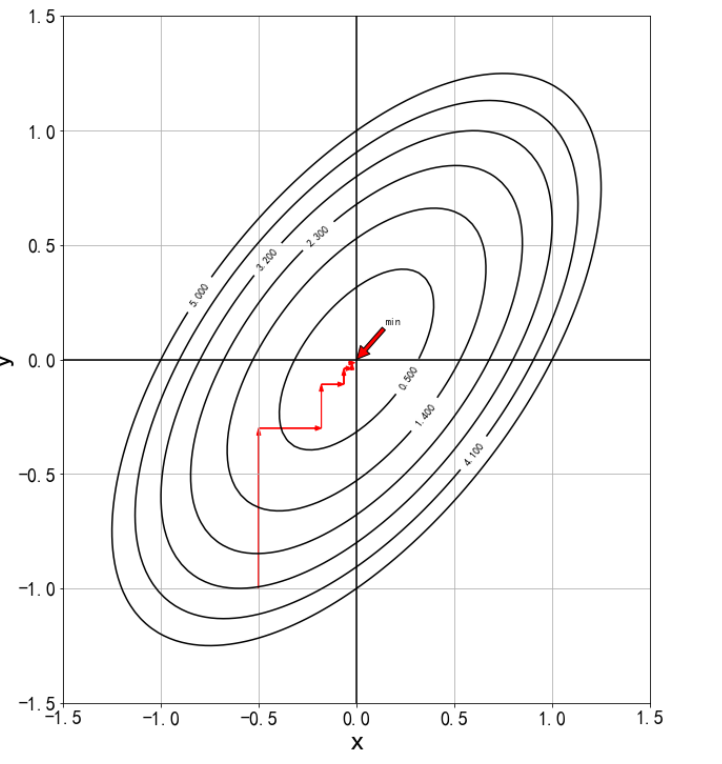
\includegraphics[height=6cm,width=9cm]{picture/00.png}
	\end{figure}
\end{frame}

\begin{frame}
	起始点(-0.5,-1.0),此时$f$=3.25。现在我们固定$x$,将$f$看成关于$y$的一元二次方程,并求当$f$最小时$y$的值:
	$$
	\begin{array}{l}
	f(x, y)=5 x^{2}-6 x y+5 y^{2}\\
	\begin{array}{l}
	f(y \mid x=-0.5)=5 *(-0.5)^{2}-6 *(-0.5) * y+5 * y^{2}+1 \\
	=5 y^{2}+3 y+1.25 \\
	f_{(y \mid x=-0.5)}^{\prime}=10 y+3=0
	\end{array}\\
	y=-0.3
	\end{array}
	$$
	所以现在自变量的值更新为(-0.5,-0.3),有$f$=0.8。
\end{frame}

\begin{frame}
	\frametitle{思考}

如果函数没有光滑性,但有凸性,收敛性是否还能成立?答案是否定的。通过图示,考虑二维的简单情况,我们就能看出这一点。
	\begin{figure}
	\centering
	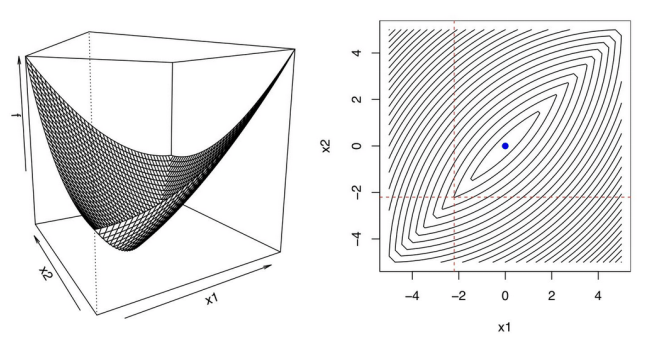
\includegraphics[height=6cm,width=9cm]{picture/01.png}
    \end{figure}
\end{frame}

\begin{frame}
	\frametitle{示例}

	难道光滑性是一个必要条件?事实上,对于一种特殊的情况
	$$
	f(x)=g(x)+\sum_{i=1}^{n} h_{i}\left(x_{i}\right)
	$$
	即$f$可以拆分成两个函数$g$和$h$,其中$g$是凸函数且光滑,$h$可以继续拆分成$h_{1},\ldots,h_{n}$($n$是$x$的维数),并且每一个$h_{i}$都是凸函数。在这种情况下,$f(x)$仍然可以通过坐标下降法求解其最小值。
\end{frame}

\begin{frame}
	\frametitle{示例}

	根据条件,我们有
	$$
	\begin{array}{l}
	f(y)-f(x) \geq \nabla g(x)^{T}(y-x)+\sum_{i=1}^{n}\left[h_{i}\left(y_{i}\right)-h_{i}\left(x_{i}\right)\right] \\
	=\sum_{i=1}^{n}\left[\nabla_{i} g(x)\left(y_{i}-x_{i}\right)+h_{i}\left(y_{i}\right)-h_{i}\left(x_{i}\right)\right] \geq 0
	\end{array}
	$$
	
\end{frame}





%\begin{frame}
%	\frametitle{示例}
%对于函数$f(x, y)=x e^{-\left(x^{2}+y^{2}\right)}$,图像如下所示:
%\begin{figure}
%	\centering
%	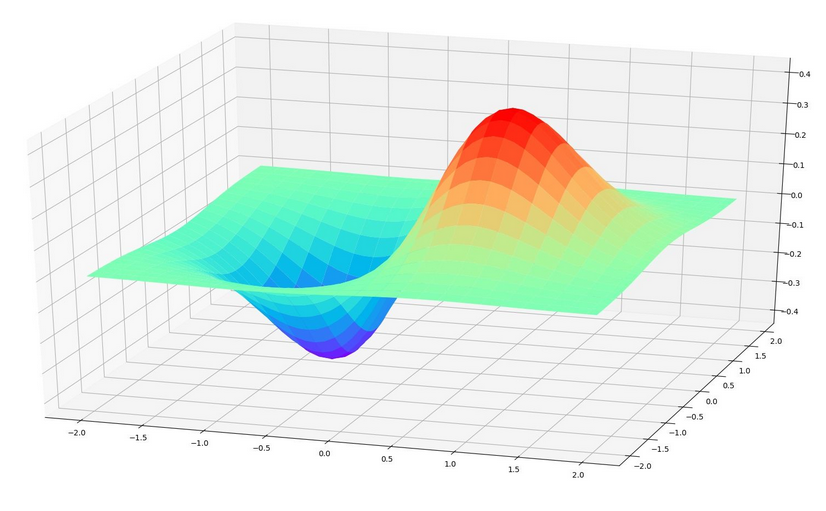
\includegraphics[height=6cm,width=9cm]{picture/3.png}
%\end{figure}
%\end{frame}
%
%\begin{frame}
%	\frametitle{示例}
%	当对其进行坐标下降的搜索结果如下图所示:
%	\begin{figure}
%		\centering
%		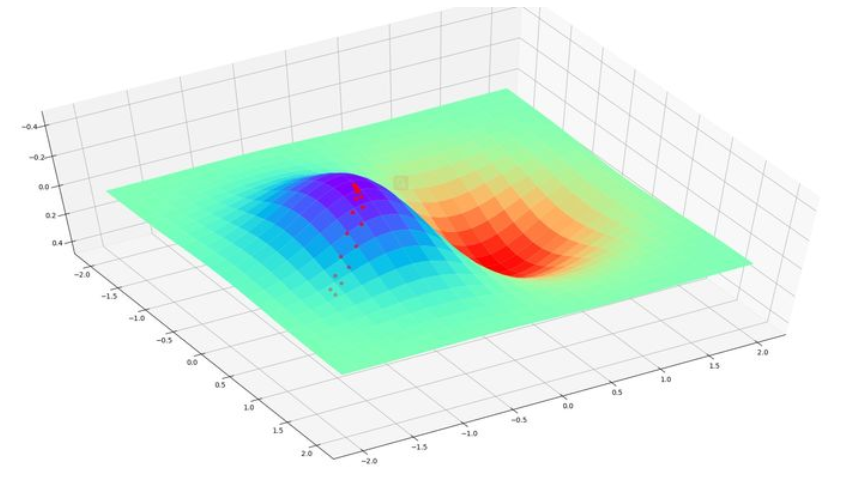
\includegraphics[height=6cm,width=9cm]{picture/4.png}
%	\end{figure}
%图中的红色小点就是搜索过程,可以看到小点是交替分布的,这也印证了坐标下降法分别在不同维度上进行交替搜索的过程。
%\end{frame}


%---------------------------------------------

%---------------------------------------------
%\begin{frame}
%\frametitle{The Logit Model}
% but its interpretation is not as simple as in ordinary linear regression because the relation is not linear, either in $z$ or $\beta_{1}$. \\
%However, we can exploit the linear relation for log odds. \\
%\bigskip
%To summarize, the logistic curve can be written as
%$$
%p(z)=\frac{\exp \left(\beta_{0}+\beta_{1} z\right)}{1+\exp \left(\beta_{0}+\beta_{1} z\right)} \quad \text { or } \quad p(z)=\frac{1}{1+\exp \left(-\beta_{0}-\beta_{1} z\right)}
%$$
%\end{frame}
%%=====================================================
\section{算法对比}

\begin{frame}
\frametitle{计算复杂度}
对于坐标下降法,如果数据的维度很大,可能需要很多次迭代。但如果运算都得当,实际是不需要的。我们不妨用线性回归的例子来对比坐标下降法和梯度下降法:
$$
\min _{\beta} \frac{1}{2}\|y-X \beta\|_{2}^{2}
$$
\end{frame}
%---------------------------------------------
\begin{frame}
	\frametitle{计算复杂度}

考虑坐标下降法。在每一个维度都取到极小值,要求$\nabla_{i} f(\beta)=0$,即
$$X_{i}^{T}(X\beta-y)=0$$
由于需要知道$\beta_{i}$的更新公式,可以先把$\beta_{i}$拆出来,也就得到
$$X\beta=X_{i}\beta_{i}+X_{-i} \beta_{-i}$$ 进一步得到$\beta_{i}$第$k+1$次迭代的更新公式
$$\beta_{i}^{k+1}=\frac{X_{i}^{T}\left(y-X_{-i} \beta_{-i}\right)}{X_{i}^{T} X_{i}}=\frac{X^{T} r}{\left\|X_{i}\right\|_{2}^{2}}+\beta_{i}^{k}$$
\end{frame}
%---------------------------------------------
\begin{frame}
	\frametitle{计算复杂度}

此外,梯度下降法的更新公式是
$$
\beta^{k+1}=\beta^{k}+t X^{T}(y-X \beta)
$$

对于梯度下降法,我们可以先计算$X \beta$,再计算$y-X \beta$,最后计算$X^{T}(y-X \beta)$,计算复杂度为$O(np)$(算出来大概是$4np$)。\\
\bigskip
对于坐标下降法,需要先更新$r$,再计算$X_{i}^{T} r$,是一个$O(n)$的复杂度,而且差不多也是$4n$的浮点数运算次数。对于$p$个维度,就是$4np$次运算。可以看出它和梯度下降法的运算次数是一样的,
\end{frame}
%---------------------------------------------
%\begin{frame}
%\frametitle{Maximum Likelihood Estimation}
%The values of the parameters that maximize the likelihood cannot be expressed in a nice closed form solution as in the normal theory linear models case.\\
%Instead they must be determined numerically by starting with an initial guess and iterating to the maximum of the likelihood function.\\
%Technically, this procedure is called an iteratively re-weighted least squares method.\\

%\end{frame}
%---------------------------------------------
\section{应用举例}
\begin{frame}
\frametitle{Lasso回归}
坐标下降法可用于求解Lasso回归。Lasso相当于带有L1正则化项的线性回归。其目标函数如下:

$$
R S S(w)+\lambda\|w\|_{1}=\sum_{i=0}^{N}\left(y_{i}-\sum_{j=0}^{D} w_{j} h_{j}\left(x_{i}\right)\right)^{2}+\lambda \sum_{j=0}^{D}\left|w_{j}\right|
$$
利用坐标下降法求解可得
$$
\hat{W}_{j}=\left\{\begin{array}{ll}
\left(p_{j}+\frac{\lambda}{2}\right) / z_{j} & , p_{j}<-\frac{\lambda}{2} \\
0 & , p_{j} \in\left[-\frac{\lambda}{2}, \frac{\lambda}{2}\right] \\
\left(p_{j}-\frac{\lambda}{2}\right) / z_{j} &, p_{j}>\frac{\lambda}{2}
\end{array}\right.
$$
其中 $p_{j}=\sum_{i=1}^{N} h_{j}\left(x_{i}\right)\left(y_{i}-\sum_{k \neq j}^{D} w_{k} h_{k}\left(x_{i}\right)\right) \quad$,$z_{j}=\sum_{i=1}^{N} h_{j}^{2}\left(x_{i}\right)$
\end{frame}
\begin{frame}
	\frametitle{Lasso回归}
利用坐标下降法求解分两步进行,先对$RSS$部分求偏导
$$
\begin{aligned}
\frac{\partial RSS(w)}{\partial w_{j}} &=-2 \sum_{i=1}^{N} h_{j}\left(x_{i}\right)\left(y_{i}-\sum_{j=0}^{D} w_{j} h_{j}\left(x_{i}\right)\right) \\
&=-2 \sum_{i-1}^{N} h_{j}(x_{i})\left(y_{i}-\sum_{k \neq j}^{D} w_{k} h_{k}\left(x_{i}\right)-W_{i} h_{j}\left(x_{i}\right)\right) \\
&=-2 \sum_{i=1}^{N} h_{j}\left(x_{i}\right)\left(y_{i}-\sum_{k\neq j}^{D} w_{k} h_{k}\left(x_{i}\right)\right)+2 W_{j} \sum_{i=1}^{N} h_{j}^{2}\left(x_{i}\right)
\end{aligned}
$$
记\\
$$
p_{j}=\sum_{i=1}^{N} h_{j}\left(x_{i}\right)\left(y_{i}-\sum_{k \neq j}^{D}w_{k} h_{k}\left(x_{i}\right)\right) \quad z_{j}=\sum_{i=1}^{N} h_{j}^{2}\left(x_{i}\right)
$$
\end{frame}

\begin{frame}
	\frametitle{Lasso回归}
$$
	\therefore \frac{\partial RSS(w)}{\partial w_{j}}=-2 p_{j}+2 w_{j} z_{j}
$$


	利用次梯度方法求解不可导部分有\\
	$$
	\lambda \partial w_{j}\left|w_{j}\right|=\left\{\begin{array}{cl}
		-\lambda & , w_{j}<0 \\
		{[-\lambda, \lambda]} & , w_{j}=0 \\
		\lambda & , w_{j}>0
	\end{array}\right.
    $$
\end{frame}

\begin{frame}
	\frametitle{Lasso回归}
	整体偏导数为:
	$$
	2 z_{j} w_{j}-2 p_{j}+\left[\begin{array}{cl}
		-\lambda & , \omega_{j}<0 \\
		{[-\lambda, \lambda]} & , w_{j}=0 \\
		\lambda & , w_{j}>0
	\end{array}\right.
	$$
	令其等于0,有
	$$
	\hat{w}_{j}=\left\{\begin{array}{ll}
	\left(p_{j}+\frac{\lambda}{2}\right) / z_{j} & , p_{j}<-\frac{\lambda}{2} \\
	0 & , p_{j} \in\left[-\frac{\lambda}{2}, \frac{\lambda}{2}\right] \\
	\left(p_{j}-\frac{\lambda}{2}\right) / z_{j} & , p_{j}>\frac{\lambda}{2}
	\end{array}\right.
	$$
	
\end{frame}
%---------------------------------------------

%---------------------------------------------

%---------------------------------------------
%\begin{frame}
%\frametitle{Likelihood Ratio Tests}
%Generally, if the null hypothesis specifies a subset of, say, $m$ parameters are simultaneously 0, the deviance is constructed for the implied reduced model and referred to a chi-squared distribution with $m$ degrees of freedom.\\
%When working with individual binary observations $Y_{\mathrm{i}}$, the residuals
%$$
%\frac{Y_{j}-\hat{p}\left(\mathbf{z}_{j}\right)}{\sqrt{\hat{p}\left(\mathbf{z}_{j}\right)\left(1-\hat{p}\left(\mathbf{z}_{j}\right)\right.}}
%$$
%each can assume only two possible values and are not particularly useful. It is better if they can be grouped into reasonable sets and a total residual calculated for each set. If there are, say, $t$ residuals in each group, sum these residuals and then divide by $\sqrt{t}$ to help keep the variances compatible.
%\end{frame}
%%=====================================================




%---------------------------------------------


%---------------------------------------------





\end{document}
